% appendixd.tex
% Dieses Werk ist unter einem Creative Commons Namensnennung-Keine kommerzielle Nutzung-Weitergabe
% unter gleichen Bedingungen 3.0 Deutschland Lizenzvertrag lizenziert. Um die Lizenz anzusehen, gehen Sie bitte
% zu http://creativecommons.org/licenses/by-nc-sa/3.0/de/ oder schicken Sie einen Brief an
% Creative Commons, 171 Second Street, Suite 300, San Francisco, California 94105, USA.


\chapter{Antworten zu ``Probiere es aus''}\label{app:answers}

%Here is where you can find the answers to the questions asked in each chapter in the section ``Things to try''.
Hier kannst du die gesamten Antworten finden, die in jedem Kapitel unter `Dinge zum ausprobieren' gestellt werden.

%%%%%%%%%%%%%%%%%%%%%%%%%%%%%%%%%%%%%%%%%%%%%%%%%%%%%%%%%%%%%%%%%%%%%%%%%%%%%%%%%%%%%%%%%
%\subsection*{Chapter \ref{ch:8multipliedby3.57}}
\subsection*{Antworten zu Kapitel~\ref{ch:8multipliedby3.57}}

%1. The answer to \textbf{Exercise 1} might be something like the following:
\subsubsection{Lösung zu Kapitel~\ref{ch:8multipliedby3.57}, Übung 1}
Die Antwort zu Kapitel~\ref{ch:8multipliedby3.57}, \textbf{Übung 1} könnte so aussehen:

%\begin{listing}
%\begin{verbatim}
%>>> toys = [ 'car', 'Nintendo Wii', 'computer', 'bike' ]
%>>> foods = [ 'pancakes', 'chocolate', 'ice cream' ]
%>>> favourites = toys + foods
%>>> print(favourites)
%['car', 'Nintendo Wii', 'computer', 'bike', 'pancakes', 'chocolate', 'ice cream']
%\end{verbatim}
%\end{listing}
\begin{Verbatim}[frame=single]
>>> spielsachen = [ 'Auto', 'Nintendo Wii', 'Computer', 'Fahrrad' ]
>>> speisen = [ 'Pfannkuchen', 'Schokolade', 'Pizza' ]
>>> favouriten = spielsachen + speisen
>>> print(favouriten)
['Auto', 'Nintendo Wii', 'Computer', 'Fahrrad', 'Pfannkuchen', 'Schokolade', 'Pizza']
\end{Verbatim}

\noindent
%2.  The answer to \textbf{Exercise 2} is simply adding the result of multiplying 3 by 25 and the result of multiplying 10 by 32.  The following equations shows the result of this equation:
\subsubsection{Lösung zu Kapitel~\ref{ch:8multipliedby3.57}, Übung 2}
Die Antwort zu \textbf{Übung 2} ist das Ergebnis von zwei Multiplikationen, deren Ergebnis miteinander addiert werden. Zuerst wird 3 mal 25 multipliziert und dann 10 mit 32. Die beiden Ergebnisse werden addiert. Die folgende Formel führt zur Lösung:

\begin{Verbatim}[frame=single]
>>> print(3 * 25 + 10 * 32)
395
\end{Verbatim}

\noindent
%However, given that we looked at the use of brackets in Chapter 2, you might have decided that you needed to put brackets around some parts of this equation.  You might've done something like this:
Aber vielleicht hast du auch Klammern verwendet, nachdem wir das in  Kapitel \ref{ch:8multipliedby3.57} so genau behandelt haben. Vielleicht hast du folgende Formel aufgeschrieben:

\begin{Verbatim}[frame=single]
>>> print((3 * 25) + (10 * 32))
395
\end{Verbatim}

\noindent
%The answer is the same, because multiplication is done before addition.  In either equation, the two multiplication operations are performed first, and the results are added.  However, the second equation is possibly slightly better than the first---because it's immediately obvious to the reader which operations are performed first.  A less knowledgeable programmer (who doesn't know as much about the order of operations) might think that, in the first equation, you multiply 3 by 25, then add 10, then multiply the result by 32 (the answer to that is 2720---completely wrong).  With the brackets, it's a bit more obvious what gets calculated first.
Das Ergebnis ist wieder das gleiche, weil die Multiplikation vor der Addition ausgeführt wird. In jeder Formel werden die zwei Multiplikationen zuerst ausgeführt und dann addiert. Aber die zweite Formel ist etwas besser als die erste---weil der Leser sofort erkennt, welche Teile zuerst berechnet werden. Jemand, der sich mit der Reihenfolge der Operatoren nicht so gut auskennt, könnte ansonsten meinen, dass in der ersten Formel 3 mit 25 multipliziert wird, dann 10 dazugezählt und das Ergebnis mit 32 multipliziert wird (das Ergebnis wäre dann 2720 und das wäre völlig falsch). Mit den Klammern wird es etwas klarer, was zuerst berechnet wird.

\noindent
%3.  The answer to \textbf{Exercise 3} will be something like the following:
\subsubsection{Lösung zu Kapitel~\ref{ch:8multipliedby3.57}, Übung 3}
Die Antwort wird ungefähr so ausschauen:

%\begin{listing}
%\begin{verbatim}
%>>> first_name = 'Mary'
%>>> second_name = 'Wilson'
%>>> print('My name is %s %s' % (first_name, second_name))
%My name is Mary Wilson
%\end{verbatim}
%\end{listing}
\begin{Verbatim}[frame=single]
>>> vorname  = 'Santa'
>>> nachname = 'Klaus'
>>> print('Mein Name ist %s %s' (vorname, nachname))
Mein Name ist Santa Klaus
\end{Verbatim}

%%%%%%%%%%%%%%%%%%%%%%%%%%%%%%%%%%%%%%%%%%%%%%%%%%%%%%%%%%%%%%%%%%%%%%%%%%%%%%%%%%%%%%%%%
%\subsection*{Chapter \ref{ch:turtles}}
\subsection*{Antworten zu Kapitel~\ref{ch:turtles}}

\noindent
%1. A rectangle is like a square, except two of its sides are longer than the other two.  By telling the turtle to do the following operations, you can easily draw a rectangle:
\subsubsection{Lösung zu Kapitel~\ref{ch:turtles}, Übung 1}
Ein Rechteck ist wie ein Quadrat, aber bei einem Rechteck sind zwei Seiten länger als die anderen zwei. So könntest du der Schildkröte befehlen ein Rechteck zu zeichnen.

%\begin{itemize}
% \item move forward a certain number of pixels
% \item turn left
% \item move forward a shorter number of pixels
% \item turn left
% \item move forward, the number of pixels in the first movement
% \item turn left
% \item move forward the shorter number of pixels in the second movement
%\end{itemize}
\begin{itemize}
 \item bewege dich um eine Anzahl von Pixel nach vorne
 \item drehe dich nach links
 \item bewege dich eine kleinere Anzahl von Pixel nach vorne
 \item drehe dich nach links
 \item bewege dich um eine Anzahl von Pixel nach vorne
 \item drehe dich nach links
 \item bewege dich eine kleinere Anzahl von Pixel nach vorne
\end{itemize}
\noindent
%For example, the following code will drawing the rectangle in figure\ref{fig46}.
Zum Beispiel würde der folgende Code das Rechteck in Abbildung~\ref{fig46} erzeugen.

%\begin{listing}
%\begin{verbatim}
%>>> import turtle
%>>> t = turtle.Pen()
%>>> t.forward(150)
%>>> t.left(90)
%>>> t.forward(50)
%>>> t.left(90)
%>>> t.forward(150)
%>>> t.left(90)
%>>> t.forward(50)
%\end{verbatim}
%\end{listing}
\begin{Verbatim}[frame=single]
>>> import turtle
>>> schildkroete = turtle.Pen()
>>> schildkroete.forward(150)
>>> schildkroete.left(90)
>>> schildkroete.forward(50)
>>> schildkroete.left(90)
>>> schildkroete.forward(150)
>>> schildkroete.left(90)
>>> schildkroete.forward(50)
\end{Verbatim}

\begin{figure}
\begin{center}
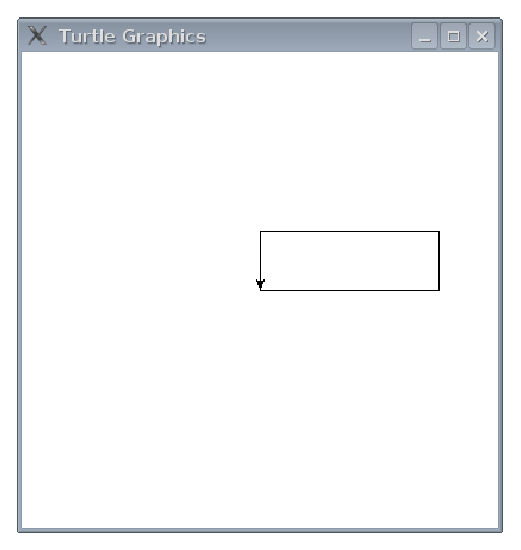
\includegraphics[width=82mm]{figure46.eps}
\end{center}
%\caption{Turtle drawing a rectangle.}\label{fig46}
\caption{Die Schildkröte malt ein Rechteck.}\label{fig46}
\end{figure}

\noindent
%2. A triangle is a bit more complicated to draw, because you need to know more about angles and line lengths.  If you haven't studied angles in school then this may be a bit harder to do than you expect.  You can draw a basic triangle (see figure~\ref{fig47}) using the following code:
Ein Dreieck zu zeichnen ist schon etwas komplizierter, weil du die Grad und die Linienlänge rausfinden musst. Wenn du noch nicht viel darüber in der Schule gehört hast, könnte das ein wenig schwerer sein. Hier wäre der Code, der das Bild in Abbildung~\ref{fig47} erzeugt:

%\begin{listing}
%\begin{verbatim}
%>>> import turtle
%>>> t = turtle.Pen()
%>>> t.forward(100)
%>>> t.left(135)
%>>> t.forward(70)
%>>> t.left(90)
%>>> t.forward(70)
%\end{verbatim}
%\end{listing}
\begin{Verbatim}[frame=single]
>>> import turtle
>>> schildkroete = turtle.Pen()
>>> schildkroete.forward(100)
>>> schildkroete.left(135)
>>> schildkroete.forward(70)
>>> schildkroete.left(90)
>>> schildkroete.forward(70)
\end{Verbatim}

%\begin{figure}
%\begin{center}
%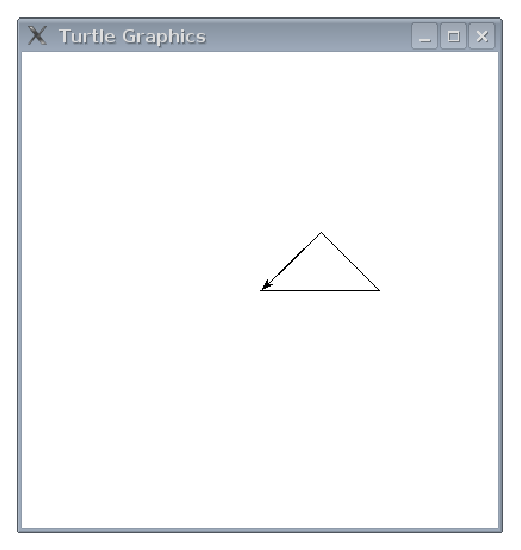
\includegraphics[width=82mm]{figure47.eps}
%\end{center}
%\caption{Turtle drawing a triangle.}\label{fig47}
%\end{figure}
\begin{figure}
\begin{center}
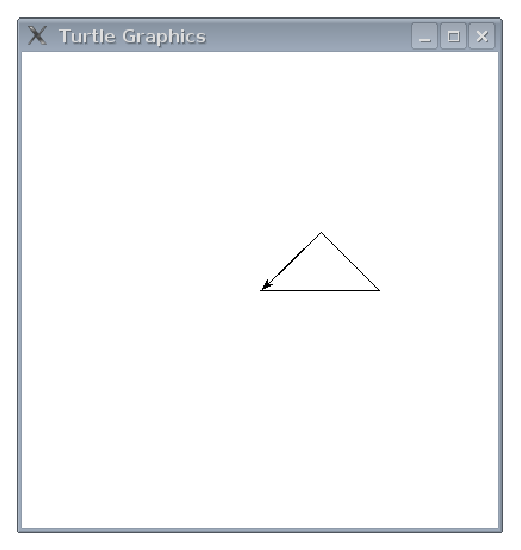
\includegraphics[width=82mm]{figure47.eps}
\end{center}
\caption{Die Schildkröte malt ein Dreieck.}\label{fig47}
\end{figure}

%%%%%%%%%%%%%%%%%%%%%%%%%%%%%%%%%%%%%%%%%%%%%%%%%%%%%%%%%%%%%%%%%%%%%%%%%%%%%%%%%%%%%%%%%
%\subsection*{Chapter \ref{ch:againandagain}}
\subsection*{Antworten zu Kapitel~\ref{ch:againandagain}}

\noindent
%1. The loop stops after the first print.  So when you run the code in the Python console you get:
\subsubsection{Lösung zu Kapitel~\ref{ch:againandagain}, Übung 1}
Die Schleife wird nach der ersten print Zeile verlassen. Also wird der Code folgendes ausgeben:

%\begin{listing}
%\begin{verbatim}
%>>> for x in range(0, 20):
%...     print('hello %s' % x)
%...     if x < 9:
%...         break
%hello 0
%\end{verbatim}
%\end{listing}
\begin{Verbatim}[frame=single]
>>> for x in range(0, 20):
...     print('Hallo %s' % x)
...     if x < 9:
...         break
...
Hallo 0
\end{Verbatim}

\noindent
%The reason it stops after the first print is that during the first run of the loop, the value of the variable \code{x} is zero.  Since zero is less than nine, the break statement stops the loop from running any further.
Der Grund, warum nur einmal etwas ausgegeben wird ist folgender: die Variable \code{x} ist am Anfang 0. Da 0 weniger als 9 ist, wird der break Befehl ausgeführt und beendet die Schleife.

\noindent
%2. To figure out how much money you get when you are paid 3\% interest, you need to multiply the number by 0.03.  To begin with we should create a variable and point it at the amount of our savings:
\subsubsection{Lösung zu Kapitel~\ref{ch:againandagain}, Übung 2}
Bei 3 Prozent Zinsen kannst du die Zinsen errechnen, indem du die Geldsumme mit 0.03 multiplizierst. Am Anfang erzeugen wir am besten eine Variable und lassen sie auf die Geldsumme zeigen.

%\begin{listing}
%\begin{verbatim}
%>>> amount = 100
%\end{verbatim}
%\end{listing}
\begin{Verbatim}[frame=single]
>>> geldsumme = 100
\end{Verbatim}

%To the amount of interest paid for 1 year would be that amount multiplied by 0.03:
Die Zinsen nach einem Jahr ergeben sich indem die Geldsumme mit 0.03 multipliziert wird:

%\begin{listing}
%\begin{verbatim}
%>>> amount = 100
%>>> print(amount * 0.03)
%3.0
%\end{verbatim}
%\end{listing}
\begin{Verbatim}[frame=single]
>>> geldsumme = 100
>>> print(geldsumme * 0.03)
3.0
\end{Verbatim}

%That's \$3!  Not bad since we didn't need to do anything to get it.  We need to print out this value and then add it to the total, and do it 10 times to work out the interest that we are paid for 10 years:
Das sind \EUR{3}! Nicht schlecht, nachdem wir nichts dafür getan haben. Jetzt geben wir diesen Wert aus, addieren ihn zur Geldsumme und berechnen die Zinsen für die größere Geldsumme von neuem. Insgesamt 10 mal.

%\begin{listing}
%\begin{verbatim}
%>>> amount = 100
%>>> for year in range(1, 11):
%...     interest = amount * 0.03
%...     print('interest earned for year %s is %s' % (year, interest))
%...     amount = amount + interest
%...
%interest earned for year 1 is 3.0
%interest earned for year 2 is 3.09
%interest earned for year 3 is 3.1827
%interest earned for year 4 is 3.278181
%interest earned for year 5 is 3.37652643
%interest earned for year 6 is 3.4778222229
%interest earned for year 7 is 3.58215688959
%interest earned for year 8 is 3.68962159627
%interest earned for year 9 is 3.80031024416
%interest earned for year 10 is 3.91431955149
%\end{verbatim}
%\end{listing}
\begin{Verbatim}[frame=single]
>>> geldsumme = 100
>>> for jahr in range(1, 11):
...     zinsen = geldsumme * 0.03
...     print('Die Zinsen für das %s Jahr sind %s' % (jahr, zinsen))
...     geldsumme = geldsumme + zinsen
...
Die Zinsen für das 1 Jahr sind 3.0
Die Zinsen für das 2 Jahr sind 3.09
Die Zinsen für das 3 Jahr sind 3.1827
Die Zinsen für das 4 Jahr sind 3.278181
Die Zinsen für das 5 Jahr sind 3.37652643
Die Zinsen für das 6 Jahr sind 3.4778222229
Die Zinsen für das 7 Jahr sind 3.58215688959
Die Zinsen für das 8 Jahr sind 3.68962159627
Die Zinsen für das 9 Jahr sind 3.80031024416
Die Zinsen für das 10 Jahr sind 3.91431955149
\end{Verbatim}

%In the first line we create a for-loop using the variable \code{year} and the function \code{range} to count from 1 to 10.  The second line calculates the interest, multiplying the value in variable \code{amount} by 0.03.  The next line is the print statement---which uses place holders (\code{\%s}) to include the values for \code{year} and \code{interest}.  Finally in the last line, we add the interest back into the amount.
In der ersten Zeile erzeugen wir eine for-Schleife mit der \code{jahr} Variable und der \code{range} Funktion, die von 1 bis 10 zählt. Die zweite Zeile berechnet die Zinsen, indem die Variable \code{geldsumme} mit 0.03 multipliziert wird. In der nächsten Zeile kommt die print Funktion mit allen Platzhaltern (\code{\%s}) damit die Werte von den Variablen \code{jahr} und \code{zinsen} eingefügt werden.
%All the decimal places---the numbers after the period (.) in the print lines---are a bit confusing, but you can tell that the amount of interest each year increases a little bit as you add the interest.
Die vielen Nachkommastellen sind vielleicht verwirrend. Aber du erkennst, wie du jedes Jahr ein wenig mehr Zinsen bekommst, da sie Geldsumme steigt.
%The code might be a bit more helpful if we also add the total saved each year:
Im nachfolgenden Code geben wir noch die Geldmenge dazu, damit du einen besseren Überblick bekommst.

%\begin{listing}
%\begin{verbatim}
%>>> amount = 100
%>>> for year in range(1, 11):
%...     interest = amount * 0.03
%...     print('interest earned for savings %s for year %s is %s' %
%...         (amount, year, interest))
%...     amount = amount + interest
%...
%interest earned for savings 100 for year 1 is 3.0
%interest earned for savings 103.0 for year 2 is 3.09
%interest earned for savings 106.09 for year 3 is 3.1827
%interest earned for savings 109.2727 for year 4 is 3.278181
%interest earned for savings 112.550881 for year 5 is 3.37652643
%interest earned for savings 115.92740743 for year 6 is 3.4778222229
%interest earned for savings 119.405229653 for year 7 is 3.58215688959
%interest earned for savings 122.987386542 for year 8 is 3.68962159627
%interest earned for savings 126.677008139 for year 9 is 3.80031024416
%interest earned for savings 130.477318383 for year 10 is 3.91431955149
%\end{verbatim}
%\end{listing}
\begin{Verbatim}[frame=single]
>>> geldsumme = 100
>>> for jahr in range(1, 11):
...     zinsen = geldsumme * 0.03
...     print('Zinsen für %s Euro im %s Jahr sind %s' % (geldsumme, jahr, zinsen))
...     geldsumme = geldsumme + zinsen
...
Zinsen für 100 Euro im 1 Jahr sind 3.0
Zinsen für 103.0 Euro im 2 Jahr sind 3.09
Zinsen für 106.09 Euro im 3 Jahr sind 3.1827
Zinsen für 109.2727 Euro im 4 Jahr sind 3.278181
Zinsen für 112.550881 Euro im 5 Jahr sind 3.37652643
Zinsen für 115.92740743 Euro im 6 Jahr sind 3.4778222229
Zinsen für 119.405229653 Euro im 7 Jahr sind 3.58215688959
Zinsen für 122.987386542 Euro im 8 Jahr sind 3.68962159627
Zinsen für 126.677008139 Euro im 9 Jahr sind 3.80031024416
Zinsen für 130.477318383 Euro im 10 Jahr sind 3.91431955149
\end{Verbatim}

%%%%%%%%%%%%%%%%%%%%%%%%%%%%%%%%%%%%%%%%%%%%%%%%%%%%%%%%%%%%%%%%%%%%%%%%%%%%%%%%%%%%%%%%%
%\subsection*{Chapter \ref{ch:sortoflikerecycling}}
\subsection*{Antworten zu Kapitel~\ref{ch:sortoflikerecycling}}

\noindent
%1. Turning the for-loop into a function is actually quite easy.  The function will look something like this:
\subsubsection{Lösung zu Kapitel~\ref{ch:sortoflikerecycling}, Übung 1}
Das Umwandelnt von einer for-Schleife in eine Funktion ist recht einfach. Die Funktion wird ungefähr so ausschauen:

%\begin{Verbatim}[frame=single]
%>>> def calculate_interest(amount, rate):
%...     for year in range(1, 11):
%...         interest = amount * rate
%...         print('interest earned for savings %s for year %s is %s' %
%...             (amount, year, interest))
%...         amount = amount + interest
%\end{Verbatim}
\begin{Verbatim}[frame=single]
>>> def berechne_zinsen(geldsumme, zinssatz):
...     for jahr in range(1, 11):
...         zinsen = geldsumme * zinssatz
...         print('Zinsen für %s Euro im %s Jahr sind %s' % (geldsumme, jahr, zinsen))
...         geldsumme = geldsumme + zinsen
...
\end{Verbatim}

%If you compare the function with the code above, you might notice that, apart from the first line, there's only one change to the original code (0.03 is now the parameter \code{rate}). Because \code{amount} was already a variable, there's no change required when it becomes a parameter. You'll find the output is also the same when you run the function:
Wenn du den Code mit der Funktion aus dem vorigen Kapitel vergleichst, fällt dir vielleicht auf, dass abgesehen von der ersten Zeile alles gleich ist (0.03 wurde jetzt zum Parameter \code{zinssatz}). Weil \code{geldsumme} schon eine Variable war, blieb da alles gleich. Die Ausgabe ist auch identisch, wenn du die Funktion verwendest:

%\begin{Verbatim}[frame=single]
%>>> calculate_interest(100, 0.03)
%interest earned for savings 100 for year 1 is 3.0
%interest earned for savings 103.0 for year 2 is 3.09
%interest earned for savings 106.09 for year 3 is 3.1827
%interest earned for savings 109.2727 for year 4 is 3.278181
%interest earned for savings 112.550881 for year 5 is 3.37652643
%interest earned for savings 115.92740743 for year 6 is 3.4778222229
%interest earned for savings 119.405229653 for year 7 is 3.58215688959
%interest earned for savings 122.987386542 for year 8 is 3.68962159627
%interest earned for savings 126.677008139 for year 9 is 3.80031024416
%interest earned for savings 130.477318383 for year 10 is 3.91431955149
%\end{Verbatim}
\begin{Verbatim}[frame=single]
>>> berechne_zinsen(100, 0.03)
Zinsen für 100 Euro im 1 Jahr sind 3.0
Zinsen für 103.0 Euro im 2 Jahr sind 3.09
Zinsen für 106.09 Euro im 3 Jahr sind 3.1827
Zinsen für 109.2727 Euro im 4 Jahr sind 3.278181
Zinsen für 112.550881 Euro im 5 Jahr sind 3.37652643
Zinsen für 115.92740743 Euro im 6 Jahr sind 3.4778222229
Zinsen für 119.405229653 Euro im 7 Jahr sind 3.58215688959
Zinsen für 122.987386542 Euro im 8 Jahr sind 3.68962159627
Zinsen für 126.677008139 Euro im 9 Jahr sind 3.80031024416
Zinsen für 130.477318383 Euro im 10 Jahr sind 3.91431955149
\end{Verbatim}


\noindent
%2. Changing the function to pass in the year as a parameter also involves only minor changes:
\subsubsection{Lösung zu Kapitel~\ref{ch:sortoflikerecycling}, Übung 2}
Die Änderung, dass auch das Jahr nun ein Parameter ist, benötigt auch nur eine kleine Anpassung:

%\begin{Verbatim}[frame=single]
%>>> def calculate_interest(amount, rate, years):
%...     for year in range(1, years):
%...         interest = amount * rate
%...         print('interest earned for savings %s for year %s is %s' %
%...             (amount, year, interest))
%...         amount = amount + interest
%\end{Verbatim}
\begin{Verbatim}[frame=single]
>>> def berechne_zinsen(geldsumme, zinssatz, jahre):
...     for jahr in range(1, jahre):
...         zinsen = geldsumme * zinssatz
...         print('Zinsen für %s Euro im %s Jahr sind %s' % (geldsumme, jahr, zinsen))
...         geldsumme = geldsumme + zinsen
...
\end{Verbatim}

\noindent
%We can now easily change the starting amount, the rate of interest and the number of years:
Nun kannst du einfach die Geldsumme, den Zinssatz und die Jahre bei jedem Aufruf der Funktion mitgeben und nach Wünschen ändern:

%\begin{Verbatim}[frame=single]
%>>> calculate_interest(1000, 0.05, 6)
%interest earned for savings 1000 for year 1 is 50.0
%interest earned for savings 1050.0 for year 2 is 52.5
%interest earned for savings 1102.5 for year 3 is 55.125
%interest earned for savings 1157.625 for year 4 is 57.88125
%interest earned for savings 1215.50625 for year 5 is 60.7753125
%\end{Verbatim}
\begin{Verbatim}[frame=single]
>>> berechne_zinsen(1000, 0.05, 6)
Zinsen für 1000 Euro im 1 Jahr sind 50.0
Zinsen für 1050.0 Euro im 2 Jahr sind 52.5
Zinsen für 1102.5 Euro im 3 Jahr sind 55.125
Zinsen für 1157.625 Euro im 4 Jahr sind 57.88125
Zinsen für 1215.50625 Euro im 5 Jahr sind 60.7753125
\end{Verbatim}


\noindent
%3. The mini-program is a bit more complicated than the functions we've already created.  First we need to import the sys module so we can ask for input.  Then we need to prompt the user of our program for each of the values.  Apart from that, the function stays roughly the same:
\subsubsection{Lösung zu Kapitel~\ref{ch:sortoflikerecycling}, Übung 3}
Dieses kleine Programm ist ein wenig komplizierter, als das bisherige. Zuerst müssen wir das \code{sys} Modul importieren um Tastatureingaben verarbeiten zu könnnen. Und wir fragen den Benutzer nach den einzelnen Werten. Sonst bleibt es gleich.

%\begin{Verbatim}[frame=single]
%>>> import sys
%>>> def calculate_interest():
%...     print('Enter the amount you have to save')
%...     amount = float(sys.stdin.readline())
%...     print('Enter the interest rate')
%...     rate = float(sys.stdin.readline())
%...     print('Enter the number of years')
%...     years = int(sys.stdin.readline())
%...     for year in range(1, years):
%...         interest = amount * rate
%...         print('interest earned for savings %s for year %s is %s' %
%...             (amount, year, interest))
%...         amount = amount + interest
%\end{Verbatim}
\begin{Verbatim}[frame=single]
>>> import sys
>>> def berechne_zinsen():
...     print('Wieviel willst du sparen?')
...     geldsumme = float(sys.stdin.readline())
...     print('Gib den Zinssatz ein')
...     zinssatz = float(sys.stdin.readline())
...     print('Wieviele Jahre bleibt das Geld auf der Bank')
...     jahre = int(sys.stdin.readline())
...     for jahr in range(1, jahre+1):
...         zinsen = geldsumme * zinssatz
...         print('Zinsen für %s Euro im %s Jahr sind %s' % (geldsumme, jahr, zinsen))
...         geldsumme = geldsumme + zinsen
...
\end{Verbatim}

\noindent
%When we run the function, we'll see something like the following:
Wenn wir die Funktion nun aufrufen bekommen wir folgendes:

%\begin{Verbatim}[frame=single]
%>>> calculate_interest()
%Enter the amount you have to save
%500
%Enter the interest rate
%0.06
%Enter the number of years
%12
%interest earned for savings 500.0 for year 1 is 30.0
%interest earned for savings 530.0 for year 2 is 31.8
%interest earned for savings 561.8 for year 3 is 33.708
%interest earned for savings 595.508 for year 4 is 35.73048
%interest earned for savings 631.23848 for year 5 is 37.8743088
%interest earned for savings 669.1127888 for year 6 is 40.146767328
%interest earned for savings 709.259556128 for year 7 is 42.5555733677
%interest earned for savings 751.815129496 for year 8 is 45.1089077697
%interest earned for savings 796.924037265 for year 9 is 47.8154422359
%interest earned for savings 844.739479501 for year 10 is 50.6843687701
%interest earned for savings 895.423848271 for year 11 is 53.7254308963
%\end{Verbatim}
\begin{Verbatim}[frame=single]
>>> berechne_zinsen()
Wieviel willst du sparen?
500
Gib den Zinssatz ein
0.06
Wieviele Jahre bleibt das Geld auf der Bank?
12
Zinsen für 500 Euro im 1 Jahr sind 30.0
Zinsen für 530.0 Euro im 2 Jahr sind 31.8
Zinsen für 561.8 Euro im 3 Jahr sind 33.708
Zinsen für 595.508 Euro im 4 Jahr sind 35.73048
Zinsen für 631.23848 Euro im 5 Jahr sind 37.8743088
Zinsen für 669.1127888 Euro im 6 Jahr sind 40.146767328
Zinsen für 709.259556128 Euro im 7 Jahr sind 42.5555733677
Zinsen für 751.815129496 Euro im 8 Jahr sind 45.1089077697
Zinsen für 796.924037265 Euro im 9 Jahr sind 47.8154422359
Zinsen für 844.739479501 Euro im 10 Jahr sind 50.6843687701
Zinsen für 844.739479501 Euro im 11 Jahr sind 53.7254308963
Zinsen für 949.149279168 Euro im 12 Jahr sind 56.9489567501
\end{Verbatim}


%%%%%%%%%%%%%%%%%%%%%%%%%%%%%%%%%%%%%%%%%%%%%%%%%%%%%%%%%%%%%%%%%%%%%%%%%%%%%%%%%%%%%%%%%
%\subsection*{Chapter \ref{ch:turtlesgalore}}
\subsection*{Antworten zu Kapitel~\ref{ch:turtlesgalore}}

\noindent
%1. There's a hard way to draw an octagon, and an easy way.  The hard way, isn't hard because it's complicated.  It's hard because it requires more typing:
\subsubsection{Lösung zu Kapitel~\ref{ch:turtlesgalore}, Übung 1}
Es gibt eine lange Variante ein Achteck zu zeichnen und eine kurze kompliziertere. Bei der langen Variante ist viel zu tippen. 

%\begin{Verbatim}[frame=single]
%import turtle
%t = turtle.Pen()
%>>> t.forward(50)
%>>> t.right(45)
%>>> t.forward(50)
%>>> t.right(45)
%>>> t.forward(50)
%>>> t.right(45)
%>>> t.forward(50)
%>>> t.right(45)
%>>> t.forward(50)
%>>> t.right(45)
%>>> t.forward(50)
%>>> t.right(45)
%>>> t.forward(50)
%>>> t.right(45)
%>>> t.forward(50)
%\end{Verbatim}
\begin{Verbatim}[frame=single]
import turtle
schildkroete = turtle.Pen()
>>> schildkroete.forward(50)
>>> schildkroete.right(45)
>>> schildkroete.forward(50)
>>> schildkroete.right(45)
>>> schildkroete.forward(50)
>>> schildkroete.right(45)
>>> schildkroete.forward(50)
>>> schildkroete.right(45)
>>> schildkroete.forward(50)
>>> schildkroete.right(45)
>>> schildkroete.forward(50)
>>> schildkroete.right(45)
>>> schildkroete.forward(50)
>>> schildkroete.right(45)
>>> schildkroete.forward(50)
\end{Verbatim}

\noindent
%You can see from that code that we tell the turtle to move forward 50 pixels, then turn right 45 degrees.  We do this 8 times.  Which is a lot of time.  The easier way to draw an octagon is the following code (which produces the octagon in figure~\ref{fig48}):
Wie du sehen kannst, sagen wir der Schildkröte, dass sie sich 50 Pixel nach vorne bewegen soll und dann 45 Grad nach rechts drehen. Wir machen das ganze 8 mal. Was ziemlich oft ist. Die kurzte Variante ist folgende (die das folgende Achteck in Bild~\ref{fig48} erzeugt):

%\begin{Verbatim}[frame=single]
%>>> for x in range(0,8):
%...     t.forward(50)
%...     t.right(45)
%\end{Verbatim}
\begin{Verbatim}[frame=single]
>>> for x in range(0,8):
...     schildkroete.forward(50)
...     schildkroete.right(45)
\end{Verbatim}

\begin{figure}
\begin{center}
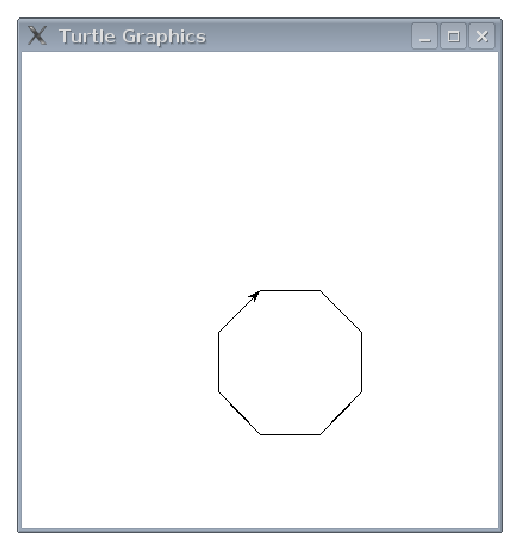
\includegraphics[width=82mm]{figure48.eps}
\end{center}
%\caption{Turtle drawing an octagon.}\label{fig48}
\caption{Die Schildkröte zeichnet ein Achteck.}\label{fig48}
\end{figure}

\noindent
%2.  If you take another look at the other functions in Chapter~\ref{ch:turtlesgalore}, you'll already see how to create a filled shape. We can convert the octagon code into a function that takes a colour, but we'll also want to reuse the hexcolour function
\subsubsection{Lösung zu Kapitel~\ref{ch:turtlesgalore}, Übung 2}
Wenn du dich nochmals in Kapitel~\ref{ch:turtlesgalore} schlau machst, findest du die Funktion, die nötig ist, um die Formen mit Farbe zu füllen. Ändern wir die \code{achteck} Funktion, damit wir gleich die Farbe mitgeben können.

%\begin{Verbatim}[frame=single]
%>>> def octagon(red, green, blue):
%...     t.color(red, green, blue)
%...     t.begin_fill()
%...     for x in range(0,8):
%...         t.forward(50)
%...         t.right(45)
%...     t.end_fill()
%\end{Verbatim}
\begin{Verbatim}[frame=single]
>>> def achteck(rot, gruen, blau):
...     schildkroete.color(rot, gruen, blau)
...     schildkroete.begin_fill()
...     for x in range(0,8):
...         schildkroete.forward(50)
...         schildkroete.right(45)
...     schildkroete.end_fill()
\end{Verbatim}

%We set the colour, then turn filling on.  Then we run the for loop to draw the octagon, finally we switch filling back off again to fill in the shape. How about a blue octagon (see figure~\ref{fig49}):
In der Funktion setzen wir die Farbe und schalten dann `ausfüllen' ein. Wir zeichnen danach das Achteck und schalten `ausfüllen' aus, um das Achteck zu füllen. Für ein blaues Achteck (siehe Bild~\ref{fig49}) geben wir folgendes ein:

%\begin{Verbatim}[frame=single]
%>>> octagon(0, 0, 1)
%\end{Verbatim}
\begin{Verbatim}[frame=single]
>>> achteck(0, 0, 1)
\end{Verbatim}

\begin{figure}
\begin{center}
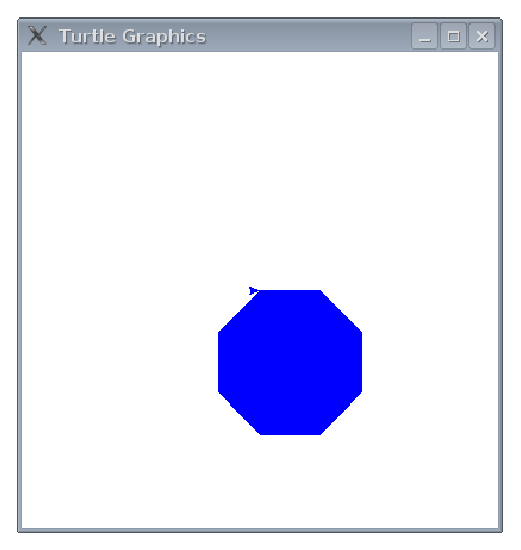
\includegraphics[width=82mm]{figure49.eps}
\end{center}
%\caption{Turtle drawing a blue octagon.}\label{fig49}
\caption{Die Schildkröte malt ein blaues Achteck.}\label{fig49}
\end{figure}
\newpage
